\section{Các bít và cách lưu trữ}

Máy tính thực chất là một máy điện, nó hoạt động dựa theo nguyên tắc lựa chọn tắt hoặc mở
hàng triệu chuyển mạch rất nhỏ bên trong nó. Các trạng thái tắt hoặc bật này được mã hoá
dưới dạng các số $0$ hoặc $1$. Các số này được gọi là các bít (gọi tắt của \textit{số nhị
  phân}).


Thông tin trong máy tính được biểu diễn dưới dạng dưới dạng dãy bít~0 hoặc~1, và dù rằng
ta nhìn các bít như giá trị số thì chúng thực sự vẫn chỉ là ký hiệu hình thức, ý nghĩa của
nó tuỳ thuộc từng cách áp dụng--lúc chúng được dùng để biển diễn giá trị số, lúc chúng
được dùng để biểu diễn ký tự trên một bảng chữ nào đó, lúc này chúng là biểu diễn hình
ảnh, lúc khác lại là biểu diễn âm thanh.

\subsection*{Phép toán Boolean}

Nếu ta xem bít $0$ biểu diễn một giá trị logic \textit{false} và bít $1$ biểu diễn cho giá
trị \textit{true} thì các thao tác bên trong máy tính có thể được mô tả một cách hình thức
bởi các \textbf{phép toán Boolean}, theo tên của George~Boole (1815-1864), một người đi
tiên phong trong Logic toán. Hình  \ref{fig:op-bool1} liệt kê ba trong nhiều phép toán
boolean: AND, OR, XOR. Các phép toán này về mặt hình thức tương tự như các phép toán hai
ngôi Nhân, Cộng và Trừ trong số học, chúng cũng nhận hai tham số đầu vào và trả ra kết
quả. Ví dụ, phép toán AND với đầu vào là cặp giá trị false~($0$) và true~($1$) sẽ cho kết
quả là false~($0$); cụ thể ta có:
\[
  0 \AND 1 = 0.
\] 
Khác ba phép toán đề cập ở trên, phép toán $\NOT$ là phép toán một ngôi, nó chỉ có một đầu
vào và một đầu ra. Trong đó đầu ra là giá trị đảo của đầu vào:
\[
\NOT  0 = 1 \mbox{ và } \NOT 1 = 0.
\]

\begin{figure}[tb]
\centering
  \begin{minipage}{1.5in}
    \begin{tabular}{cc|c}
      $p$ & $q$ & $p \AND q$ \\
      \hline
      0 & 0 & 0 \\
      0 & 1 & 0 \\
      1 & 0 & 0 \\
      1 & 1 & 1
    \end{tabular}
  \end{minipage}
  \begin{minipage}{1.5in}
    \begin{tabular}{cc|c}
      $p$ & $q$ & $p \OR q$ \\
      \hline
      0 & 0 & 0 \\
      0 & 1 & 1 \\
      1 & 0 & 1 \\
      1 & 1 & 1
    \end{tabular}
  \end{minipage}
  \begin{minipage}{1.5in}
    \begin{tabular}{cc|c}
      $p$ & $q$ & $p \XOR q$ \\
      \hline
      0 & 0 & 0 \\
      0 & 1 & 1 \\
      1 & 0 & 1 \\
      1 & 1 & 0
    \end{tabular}
  \end{minipage}
  \caption{Các phép toán AND, OR, XOR (tuyển loại). Hai cột đầu tiên biểu diễn tham số đầu
    vào, cột thứ ba chỉ kết quả của phép toán tương ứng với tham số đó.}
    \label{fig:op-bool1}
\end{figure}

\subsection*{Các cổng logic và Flip-Flop} 

%Các kết quả của đại số Boolean rất quan trọng trong thiết kế các thành phần của máy tính. Ý tưởng cơ bản là xây dựng các mạch đơn giản thực hiện một vài phép toán Boolean, còn các mạch phức tạp hơn có thể xây dựng lại được bằng cách kết hợp các mạch đơn giản đó.

\begin{figure}[tbh]  
\centering

\subfloat[Cổng logic $\AND$]{
  \begin{minipage}{3in}
\begin{center}
    \scalebox{0.5}{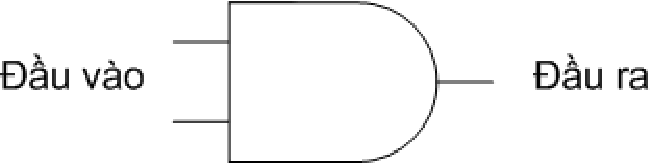
\includegraphics{ch2/fig2and.pdf}}

    \vspace{0.5cm}
    \begin{tabular}{cc|c}
      \multicolumn{2}{c|}{Đầu vào} &  Đầu ra \\
      \hline
      0 & 0 & 0 \\
      0 & 1 & 0 \\
      1 & 0 & 0 \\
      1 & 1 & 1
    \end{tabular}
  \end{center}
\end{minipage}
}
\subfloat[Cổng logic $\OR$]{
  \begin{minipage}{3in}
    \begin{center}
      \scalebox{0.5}{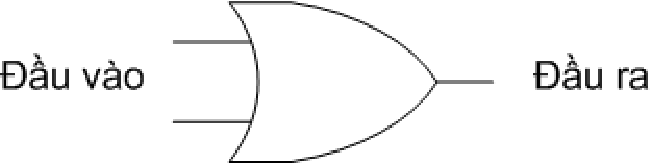
\includegraphics{ch2/fig2or.pdf}} 

      \vspace{0.5cm}
      \begin{tabular}{cc|c}
      \multicolumn{2}{c|}{Đầu vào} &  Đầu ra \\
      \hline
      0 & 0 & 0 \\
      0 & 1 & 1 \\
      1 & 0 & 1 \\
      1 & 1 & 1
    \end{tabular}
  \end{center}
\end{minipage}
}

\vspace{0.7cm}

\subfloat[Cổng logic $\XOR$]{
  \begin{minipage}{3in}
    \begin{center}
      \scalebox{0.5}{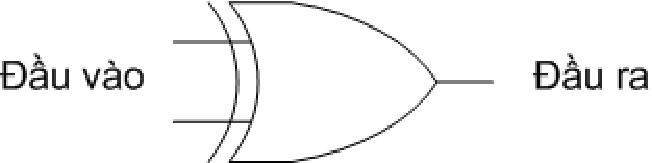
\includegraphics{ch2/fig2xor.pdf}}

      \vspace{0.5cm}
      \begin{tabular}{cc|c}
        \multicolumn{2}{c|}{Đầu vào} &  Đầu ra \\
        \hline
        0 & 0 & 0 \\
        0 & 1 & 1 \\
        1 & 0 & 1 \\
        1 & 1 & 0
      \end{tabular}
    \end{center}
\end{minipage}
}
\subfloat[Cổng logic $\NOT$]{
  \begin{minipage}{3in}
    \begin{center}
      \scalebox{0.5}{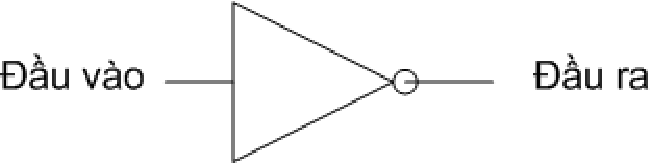
\includegraphics{ch2/fig2not.pdf}} 

\vspace{0.5cm}
      \begin{tabular}{c|c}
        Đầu vào &  Đầu ra \\
        \hline
        0 & 0 \\
        1  & 0 
      \end{tabular}
    \end{center}
  \end{minipage}
} 

\vspace{0.3cm}
\caption{Các cổng logic}
\label{fig:op-bool2}
\end{figure}


\begin{figure}[tbh]  
\centering
    \scalebox{0.4}{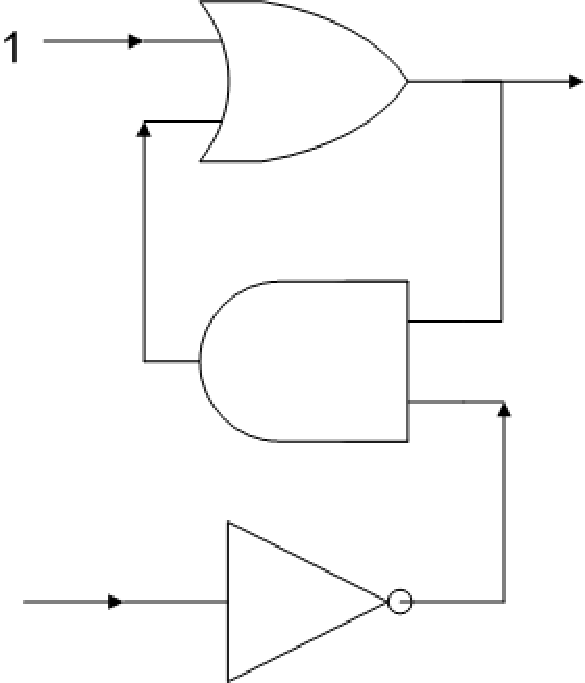
\includegraphics{ch2/fig-fflp.pdf}}
\caption{Một mạch Flip-Flop}
 \label{fig:op-flipflop}
\end{figure}
 

\textbf{Cổng} là một thiết bị điện tử có một hoặc nhiều đầu vào, mỗi đầu vào nhận giá trị
$0$ hoặc~$1$, tương ứng với hai mức điện thế; và thường có một đầu ra, đó là một hàm theo
đầu vào, nó cũng nhận giá trị~$0$ hoặc~$1$.  Trong giáo trình này, ta sẽ chỉ xem xét một
cách hình thức các cổng như các ký hiệu, bỏ qua cách biểu diễn vật lý của chúng.

Một cổng thường để tính toán một hàm Boolean cụ thể, đơn giản nào đó. Trong nghành công
nghiệp điện tử, người ta thường chỉ xây dựng một số cổng thực hiện một vài hàm nhất định,
còn các hàm khác sẽ được xây dựng lại bằng cách tổ hợp các cổng cơ bản đó.  Một số cổng
quen thuộc được liệt kê trong Hình~\ref{fig:op-bool2}.

 
Các cổng được tổ hợp thành các \textbf{mạch số} (gọi tắt là mạch) bằng cách nối đầu ra của
một số cổng với đầu vào một số cổng khác. Mỗi mạch có thể có một hoặc nhiều đầu vào, mỗi
đầu vào này lại có thể là đầu vào của nhiều cổng khác bên trong mạch. Đầu ra của mạch là đầu ra của một hoặc
nhiều cổng trong mạch.

Một mạch quan trọng trong thiết kế các phần tử nhớ được chỉ ra trong Hình~\ref{fig:op-flipflop}, nó được gọi là mạch Flip-Flop. Một Flip-Flop là một mạch được thiết
kế để giữ giá trị đầu ra ($0$ hoặc~$1$) không thay đổi cho tới khi nhận được tín hiệu từ
đầu vào yêu cầu chuyển sang một giá trị khác. Để ý rằng, khác với các phép toán Boolean
trước, giá trị đầu ra của mạch kiểu này không chỉ phụ thuộc đầu vào ở thời điểm hiện tại
mà còn phụ thuộc cả vào đầu ra của thời điểm trước nữa.

Ta khẳng định rằng: khi cả hai giá trị đầu vào của mạch trong Hình \ref{fig:op-flipflop}
đều là~$0$ thì đầu ra của mạch không thay đổi (dù nó có là $0$ hay $1$). Tuy nhiên, khi ta
đặt giá trị $1$ cho đầu vào phía trên của mạch, ngay lập tức đầu ra sẽ là~$1$. Còn khi ta
đặt giá trị $1$ cho đầu vào phía dưới, ngay lập tức đầu ra của mạch sẽ là $0$.


\begin{figure}[tbh] 
\centering
\subfloat[Đặt $1$ và $0$ vào 2 đầu vào]{
    \scalebox{0.35}{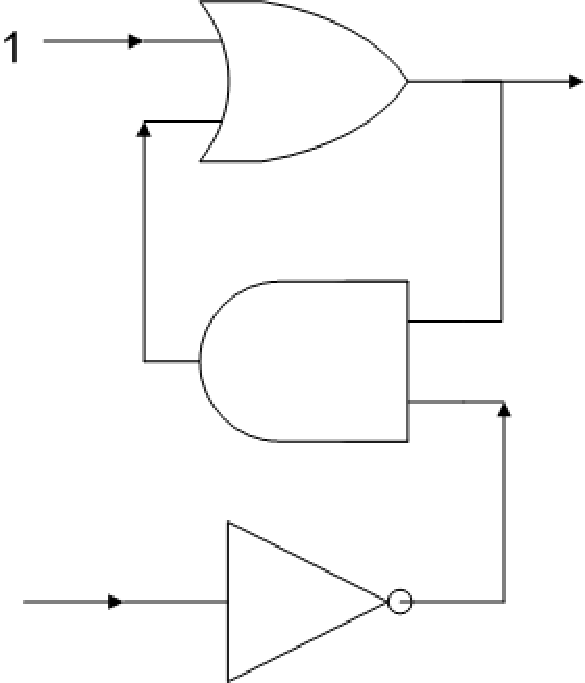
\includegraphics{ch2/figffl1.pdf}}
\label{op-flipflop2a}
}\qquad \subfloat[Đầu ra của cổng $\OR$ và cổng $\AND$ đều là $1$]{
  \scalebox{0.35}{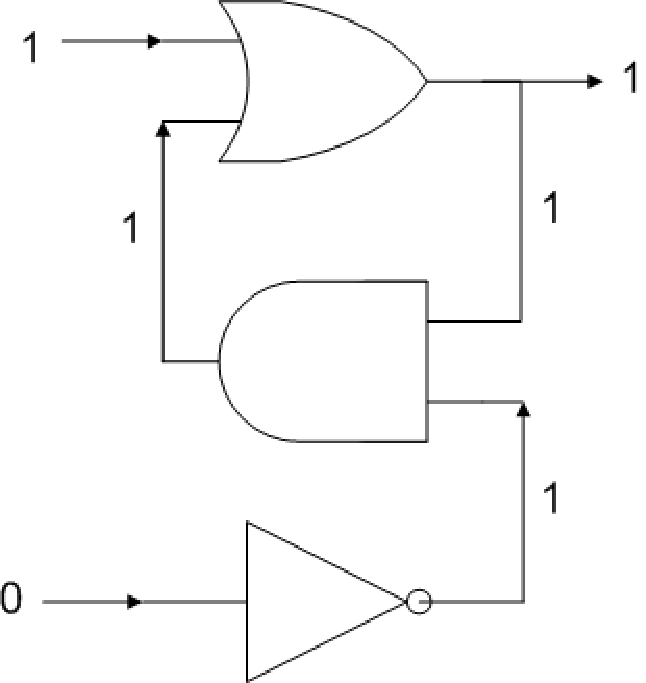
\includegraphics{ch2/figffl2.pdf}}
\label{op-flipflop2b}
} \qquad \subfloat[Giá trị $1$ từ cổng $\AND$ giữ cho đầu ra của $\OR$
bằng $1$ dù đầu vào kia bằng $0$]{
  \scalebox{0.35}{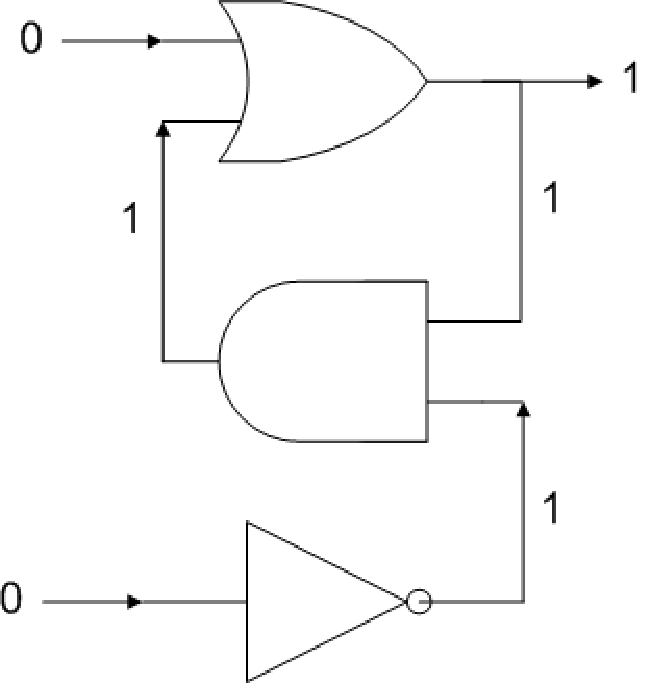
\includegraphics{ch2/figffl3.pdf}}
\label{op-flipflop2c}
}
\caption{Đưa giá trị đầu ra của Flip-Flop lên 1}
\label{fig:op-flipflop2}
\end{figure}

Ta sẽ cùng phân tích khẳng định trên một cách chi tiết. Trước hết, ta thấy rằng dù đầu ra
của mạch~\ref{fig:op-flipflop} là gì đi nữa, nếu đầu vào phía trên của mạch đặt
bằng~$1$ và phía dưới đặt bằng $0$, vậy đầu ra của cổng $\OR$ sẽ là~$1$. Bây giờ, cả hai
đầu vào của cổng $\AND$ đều bằng $1$, vậy đầu ra của nó bằng $1$, có nghĩa rằng đầu vào
thứ hai của $\OR$ sẽ là~$1$ (Hình~\ref{op-flipflop2b}). Điều này làm cho đầu ra của $\OR$
vẫn bằng $1$, kể cả khi bây giờ đầu vào phía trên của mạch được đặt bằng $0$ (Hình~\ref{op-flipflop2c}).  Tóm lại, đầu ra của Flip-Flop đã trở thành $1$ và luôn giữ ở giá
trị đó dù đầu vào phía trên được đặt bằng $0$ hay không.
 

Cũng tương tự như trên, khi đặt giá trị $1$ cho đầu vào phía dưới sẽ làm cho đầu ra của
Flip-Flop là $0$ và giá trị này vẫn giữ nguyên khi giá trị đầu vào được đưa trở về~$0$.
   
Ta trình bày mạch Flip-Flop trong Hình~\ref{fig:op-flipflop} và Hình~\ref{fig:op-flipflop2}
với hai mục đích. Thứ nhất, nó chỉ ra làm thế nào các thiết bị có thể được xây dựng từ
các cổng, quá trình này được gọi là thiết kế mạch số, nó đóng vai trò quan trọng trong
nghành công nghệ máy tính. Thứ hai, nó cho ta cách để lưu trữ một bít trong máy tính. Thật
vậy, mạch Flip-Flop cho phép ta đặt giá trị để đầu ra của nó luôn bằng $0$ hoặc bằng
$1$. Vậy các mạch khác muốn lưu trữ có thể gửi tín hiệu tới đầu vào của Flip-Flop để đặt
giá trị, và các mạch khác nữa có thể sử dụng giá trị lưu trữ bằng cách lấy giá trị từ đầu
ra của Flip-Flop như đầu vào của nó. Với kỹ thuật hiện nay, rất nhiều Flip-Flop có thể
được kết hợp lại trong một chip và được sử dụng để lưu trữ thông tin dưới dạng mã hoá như
dãy bít~$0$ và~$1$.

\subsection*{Bài tập}
\begin{enumerate}
 \item Với những giá trị đầu vào nào thì mạch sau đây cho đầu ra là $1$?
    \begin{center}
      \scalebox{0.55}{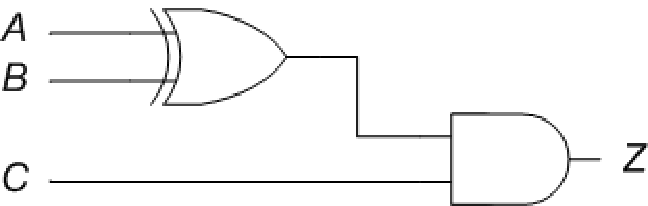
\includegraphics{ch2/bt1.pdf}}
    \end{center}

 \item Phần trình bày ở trên khẳng định rằng việc đặt $1$ cho đầu vào
   phía dưới của Flip-Flop trong Hình~\ref{fig:op-flipflop} (trong khi
   vẫn giữ đầu vào phía trên bằng $0$) sẽ làm cho đầu ra của Flip-Flop
   bằng $0$. Hãy mô tả dãy các sự kiện xuất hiện trong Flip-Flop trong
   trường hợp này?

  \item Một cách xây dựng Flip-Flop khác được chỉ ra bởi hình dưới đây. Giả sử rằng cả hai
    đầu vào của Flip-Flop này là $0$, hãy mô tả dãy các sự kiện xuất hiện khi cho đầu vào
    phía trên giá trị $1$.
   \begin{center}
     \scalebox{0.6}{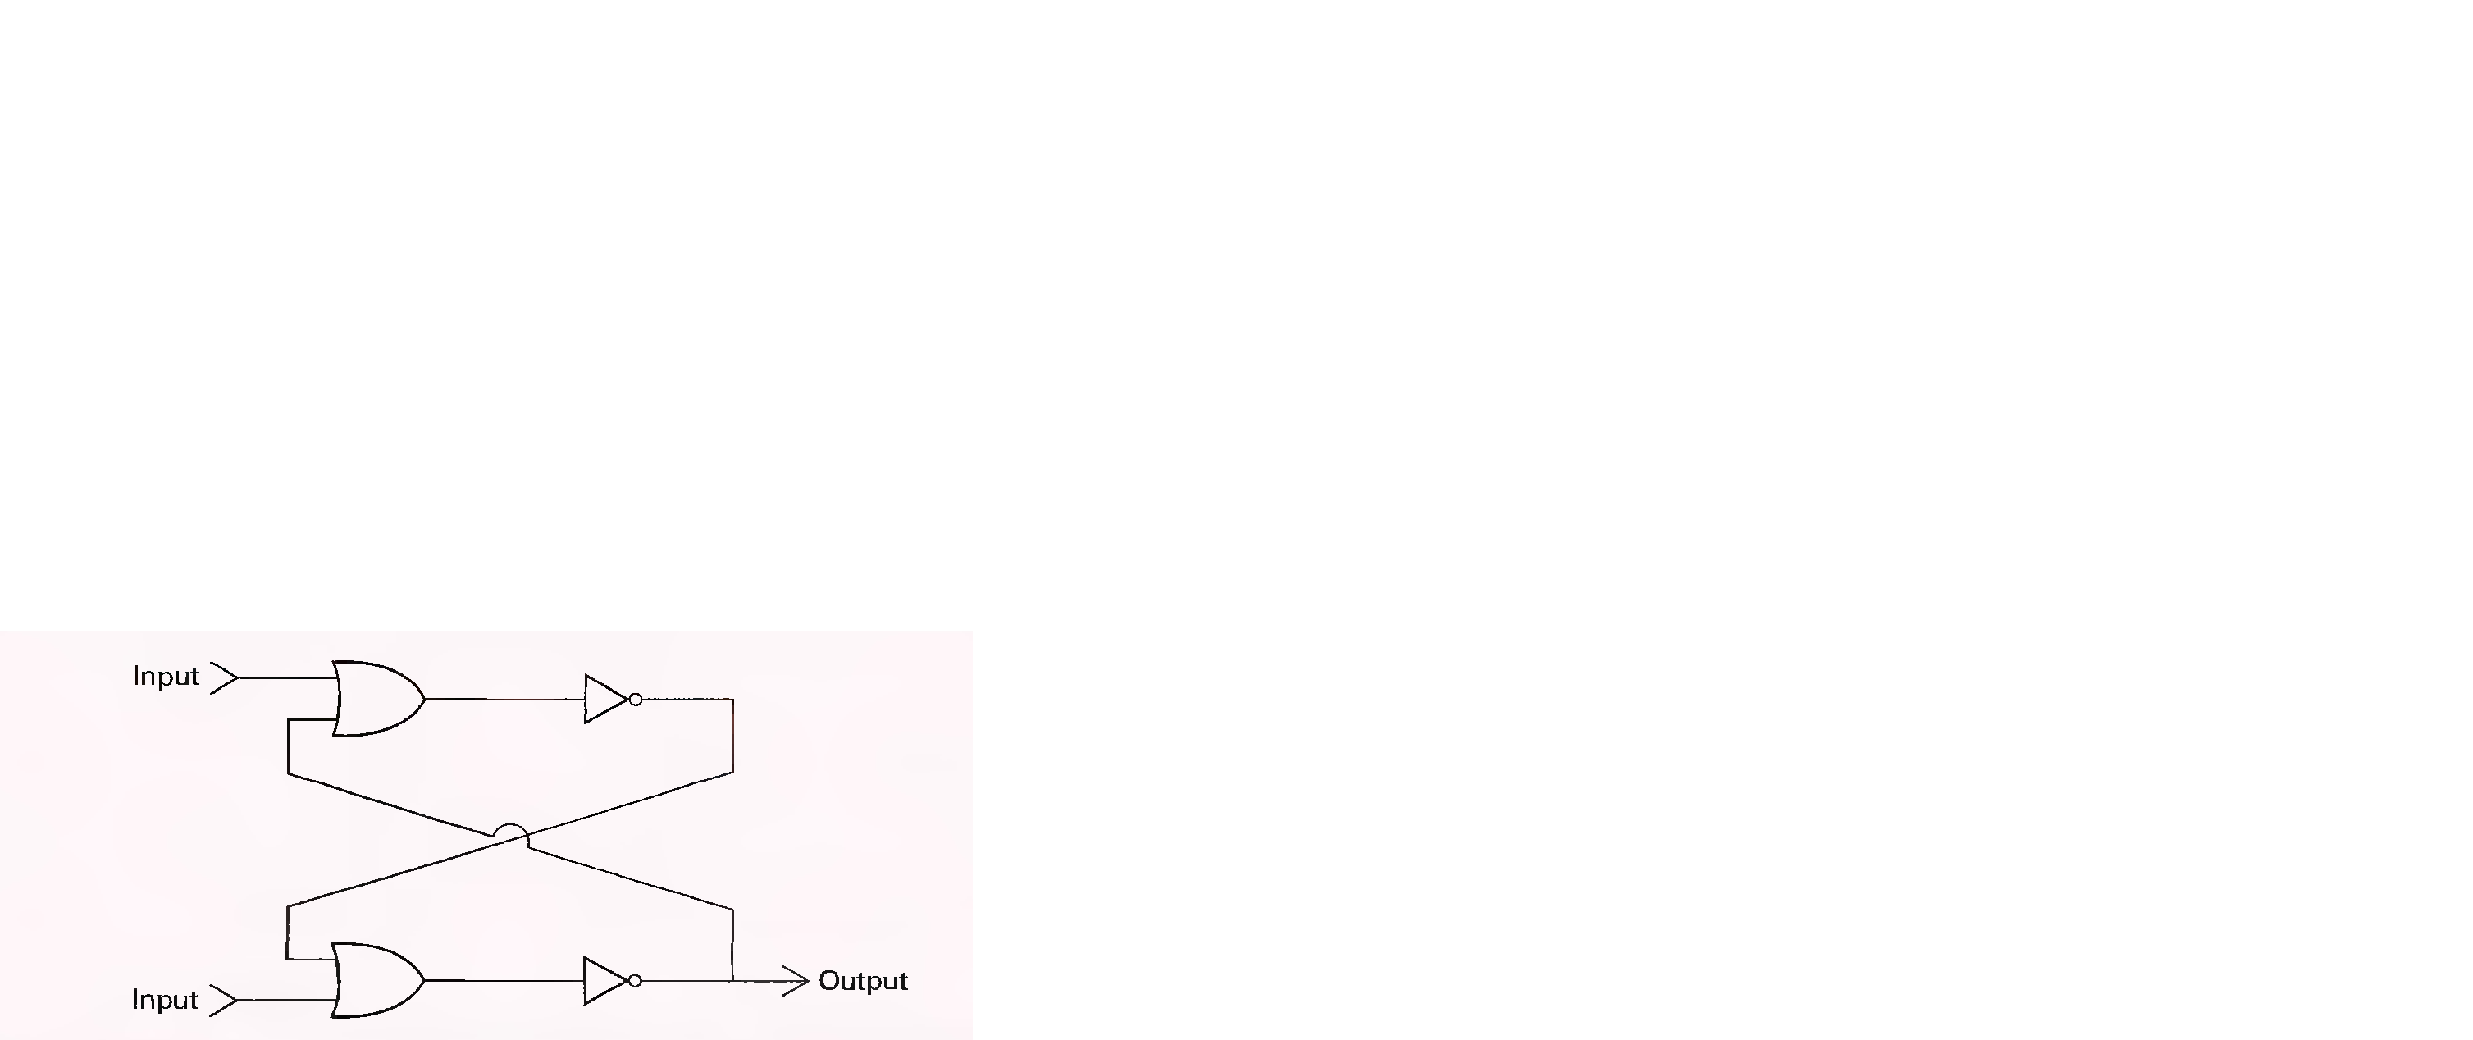
\includegraphics{ch2/fig15.pdf}}
   \end{center}


 \item Phối hợp các hoạt động của các thành phần khác nhau bên trong
   máy tính là rất cần thiết. Điều này được làm bằng cách nối với một
   xung đồng hồ với các mạch cần phối hợp.  Bởi vì đồng hồ thay đổi
   luân phiên giữa giá trị $0$ và $1$, nó làm cho các thành phần mạch
   hoạt động. Dưới đây là một ví dụ một phần của mạch liên quan đến
   Flip-Flop trong Hình~\ref{fig:op-flipflop}. Giá trị nào của xung
   đồng hồ sẽ chặn các giá trị đầu vào của mạch tác động đến
   Flip-Flop? Giá trị nào của xung đồng hồ sẽ làm cho Flip-Flop phản
   ứng lại với giá trị đầu vào của mạch?
    \begin{center}
      \scalebox{0.55}{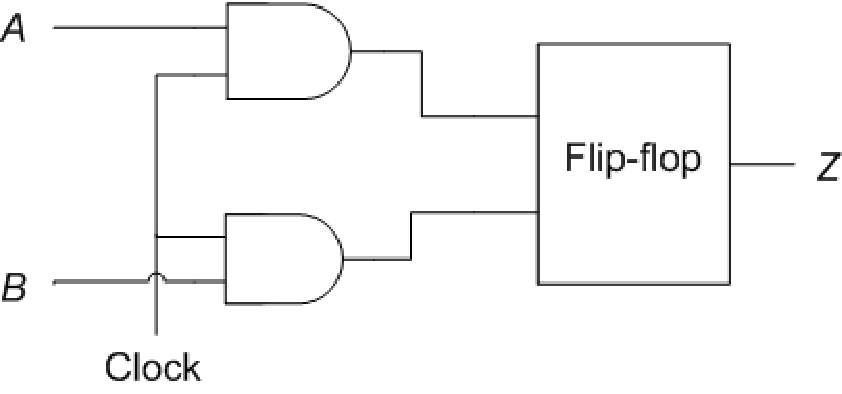
\includegraphics{ch2/bt4.pdf}}
    \end{center}

\item
  \begin{enumerate}
  \item Nếu đầu ra của cổng $\OR$ được nối với cổng $\NOT$, ta gọi nó
    là mạch $\NOR$. Mạch này có đầu ra là $1$ chỉ khi cả hai đầu vào
    đều có giá trị $0$. Ta ký hiệu cổng này cũng giống cổng $\OR$
    nhưng thêm một vòng tròn ở đầu ra của nó. Mạch dưới đây bao gồm
    một cổng $\AND$ và hai cổng $\NOR$. Hãy mô tả phép toán Boolean mà
    mạch này tính?
%\begin{figure}[h]
    \begin{center}
      \scalebox{0.55}{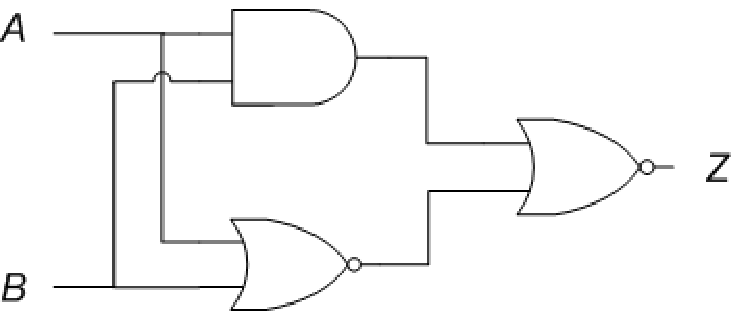
\includegraphics{ch2/bt5a.pdf}}
    \end{center}
%\caption{Một mạch Flip-Flop}
%  \label{fig:op-flipflop}
%\end{figure}

  \item Nếu đầu ra của cổng $\AND$ được nối với cổng $\NOT$, ta gọi nó
    là mạch $\NAND$.  Mạch này có đầu ra là $0$ chỉ khi cả hai đầu vào
    đều có giá trị $1$. Ta ký hiệu cổng này cũng giống cổng $\AND$
    nhưng thêm một vòng tròn ở đầu ra của nó. Mạch dưới đây bao gồm
    các cổng $\NAND$. Hãy mô tả phép toán Boolean mà mạch này tính?
    \begin{center}
      \scalebox{0.55}{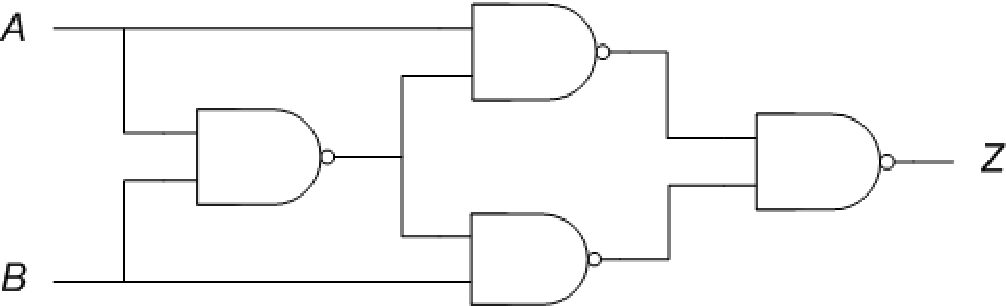
\includegraphics{ch2/bt5b.pdf}}
    \end{center}

  \end{enumerate}
\end{enumerate}

%%% Local Variables: 
%%% mode: latex
%%% TeX-master: "../tindaicuong"
%%% End: 
